In this chapter, we describe the details about the implementation of our approach to create the dynamic benchmark. The source code of this implementation is present on GitHub at \url{https://github.com/sola-st/master-thesis-piyush-bajaj/tree/automation}
We use various tools and libraries to make the benchmark accomplish the goals of being ready-to-run, ready-to-analyze, versatile, extensible and diverse and large-scale.
We describe these tools and libraries in the following sections.

\section{Source for Corpus of Projects}
\label{impl:corpus of projects}
As mentioned in the approach, we select the projects belonging to the different application domains from a predefined set of 679 projects from the the awesome python project.
In this work, we use the table of contents as shown in the Figure \ref{fig:awesome-python-website} to be the application domain for our selection process.
The figure \ref{fig:awesome-python-website} also shows the projects listed under the categories of Email, Enterprise Application Integration and Environment Management.
The category of Email further breaks down the projects into 3 sub-categories of Mail Servers, Clients and Others.
The GitHub repository of awesome python as well as the accompanying website can be accessed at \url{https://github.com/vinta/awesome-python/}.
We get source code of the project from GitHub repository which is provided by awesome python or the project website.  

\begin{figure}
    \centering
    \includegraphics[width=1\linewidth, height=1\linewidth]{figures/implementation/Awesome-Python-website3.png}
    \caption{Awesome Python Website}
    \label{fig:awesome-python-website}
\end{figure}

\section{First 5 Projects}
\label{impl:first five}
We start by manually selecting a random project from one of the categories in the awesome python corpus.
Then the number of stars for the repository on GitHub is checked. 
If the project has less than 500 stars we choose another random project, otherwise we proceed with the selected project.
This helps us to ensure the GitHub stars selection criteria mentioned in section \ref{approach:selection criteria}.
We proceed by cloning the source code of the project and installing it in a python virtual environment.
If the project is successfully installed, we add the pytest library to the virtual environment.
Finally, the test suite of the project is run using pytest. 
The project is chosen only if the execution is successful ensuring the selection criteria of presence and execution of test suite is met.

All of the above mentioned steps, from selecting a random project to running the test suite is performed a number of times to collect 5 different projects. 
Each time a random project is selected, we ensure that it does not belong to any of the categories that have been chosen before.
This helps us fulfill the selection criteria of diverse domain mentioned in section \ref{approach:selection criteria}.
Some library and dependency requirements were fixed during installation and execution of the projects.
Table \ref{table:first_5_projects} shows a list the projects which were chosen for installation till 5 of them satisfied all the selection criteria.

\begin{table}[ht]
    \centering
    \begin{tabular}{lllll}
    \hline
    \textbf{Category} & \textbf{Sub-category} & \textbf{Name} & \textbf{GitHub Stars} & \textbf{Criteria}\\
    \hline
    Web Crawling & - & grab & 2.2k & Yes\\
    DevOps Tools & SSH-style Deployment & fabric & 13.7k & No\\
    Robotics & - & PythonRobotics & 16.8k & Yes\\
    RESTful API & Flask & flask-api & 1.3k & Yes\\
    Deep Learning & - & mxnet & 20.2k & No\\
    Machine Learning & - & gym & 29k & No\\
    Job Scheduler & - & schedule & 10.2k & Yes\\
    Image processing & - & pagan & 278 & No\\
    Image Processing & - & pillow & 10.3k & Yes\\
    \hline
    \end{tabular}
    \caption{First 5 Projects for DyPyBench (Criteria : Test Suite Execution)}
    \label{table:first_5_projects}
\end{table}

\section{Automation for Installation}
\label{impl:automation}
Manual installation of projects as described in section \ref{impl:first five} shows us that the tasks of installation and execution are repetitive for each project with some exceptions.
These tasks become tedious and error prone, when we need to repeat them for 50 projects.
We automate these tasks using bash scripts which support loops for repetition and exceptions using conditionals.
The Figure \ref{fig:setup difference} shows the installation steps for two projects that satisfied the selection criteria.
The blue colored text indicate similarities, whereas the red colored text indicate the differences.

\begin{figure}[ht]
    \centering
    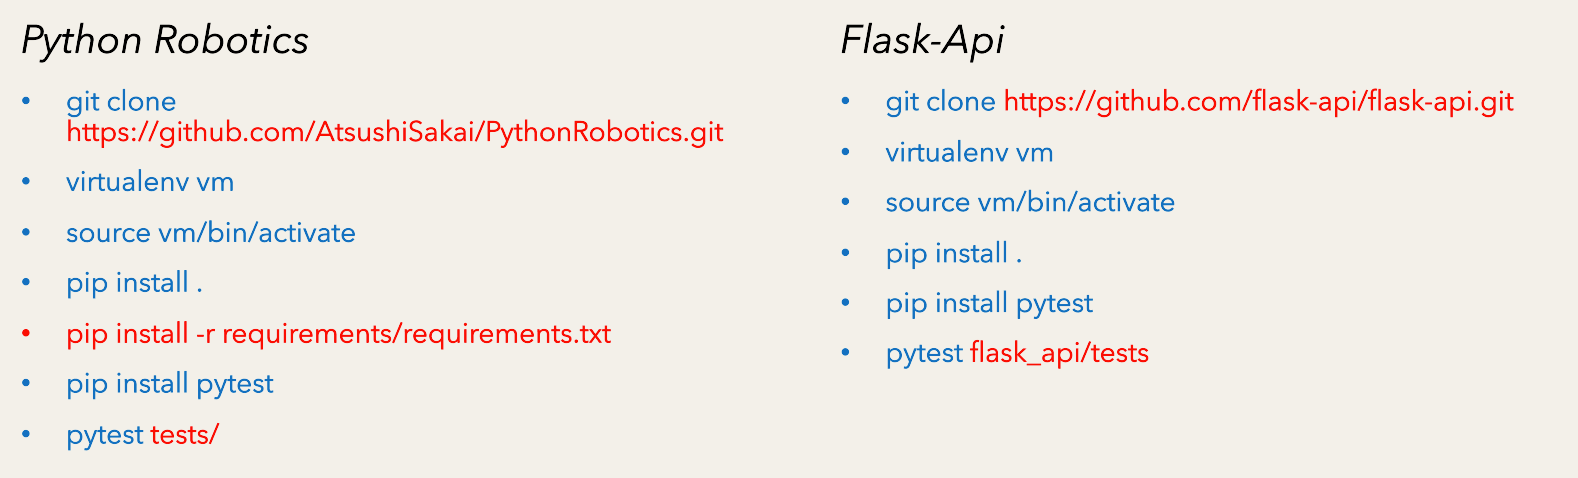
\includegraphics[width=1\linewidth]{figures/implementation/Setup-difference.png}
    \caption{Execution of Projects (Similarities and Differences)}
    \label{fig:setup difference}
\end{figure}

As can be seen from the Figure \ref{fig:setup difference}, the two commands of \textbf{git clone} and \textbf{pytest} have different argument values depending on the project.
To handle these difference we provide arguments to the bash script based on the project thereby making the automation generic.
These arguments are present in a text file, which is read by the bash script and the commands are run with the given arguments.
This text file is named as github-url.txt and contains a separate line for each project consisting of the GitHub URL and test directory path from the project root.
Furthermore, as can be seen from the Figure \ref{fig:setup difference}, Python Robotics project runs an extra command.
Execution of this command varies based on the presence or absence of the requirements file.
To handle this difference, github-url.txt file also contains a flag value for the project.
The flag value of \textit{rt} specifies the presence of requirements file, whereas the value \textit{t} indicates its absence.
We specify the path of the relevant requirements file for the project in case the flag value is \textit{rt}.
The Listing \ref{code:github-url-2} shows the entry of two projects shown in the Figure \ref{fig:setup difference}.

\lstset{numbers=left, numberstyle=\tiny, stepnumber=1, numbersep=5pt, columns=flexible, breaklines=true}
\lstset{basicstyle=\ttfamily}
\lstset{frame=tb}

\begin{lstlisting}[float,caption=Sample Entry github-url.txt,label=code:github-url-2,language=Bash]
https://github.com/AtsushiSakai/PythonRobotics.git rt requirements/requirements.txt tests
https://github.com/flask-api/flask-api.git t flask_api/tests
\end{lstlisting}

The bash script to automate the steps of installation of the 5 projects in section \ref{impl:first five} is shown in the Listing \ref{code:install-all-projects.sh}.
All the commands for installation shown in the Figure \ref{fig:setup difference} are present in this script.
We start by creating a common directory for all projects. 
Then we read the github-url.txt and loop over each line in the file indicated on line 20.
We split the line into parts to obtain the required argument for the concerned command.
Inside the folder created for each project, we clone the GitHub repository using the git clone command as shown on line 33.
After cloning the repository, we create the virtual environment and activate it as shown in lines 37 through 41.
Then the project is installed using pip as shown on the line 53.
This installs the project from the source code.
Next, on line 55 we check flag value for requirements file.
If present we install the dependencies from requirements file specified by its path on line 58.
On line 64, we install some dependencies for running the project test suite as these were missed during the installation.
We then finally install pytest library on line 68 and deactivate the virtual environment. 

\lstset{numbers=left, numberstyle=\tiny, stepnumber=1, numbersep=5pt, columns=flexible, breaklines=true, numberblanklines=false}
\lstset{basicstyle=\ttfamily}
\lstset{frame=tb}

\begin{lstlisting}[caption=Bash Script for Automation,label=code:install-all-projects.sh,language=Bash]
#root directory
ROOT_DIR=/DyPyBench
cd $ROOT_DIR

#read URL_FILE
URL_FILE=$ROOT_DIR/text/github-url.txt

# Create project folder to keep all the projects together inside one parent folder
PROJ_DIR=$ROOT_DIR/../Project
#if folder already present, then delete the folder
if [ -d "$PROJ_DIR" ]
then
    rm -rf "$PROJ_DIR" 
fi
mkdir -p "$PROJ_DIR"
cd "$PROJ_DIR"

#run a while loop for all projects
idx=1
while read line
do
    parts=($line)
    URL=${parts[0]}
    FLAGS=${parts[1]}
    
    #change to working directory
    cd $PROJ_DIR
    
    #create directory for project
    mkdir -p "project$idx"
    
    #clone the repo to project directory
    git clone "$URL" "project$idx"
    cd "project$idx"
    
    #create virtual env name .vm
    virtualenv .vm
    
    #activate virtual env
    if [[ -d ".vm/local" ]]
    then
        source .vm/local/bin/activate
    elif [[ -d ".vm/bin" ]]
    then
        source .vm/bin/activate
    else
        echo "Unable to create virtual env"
        exit
    fi

    #install using pip install . 
    echo "Running pip install ."
    pip install .

    if [[ $FLAGS == "rt" ]]
    then
        echo "Running pip install requirements"
        pip install -r $REQ_FILE
    fi

    #some projects need extra requirements for running test suites
    if [[ $URL == "https://github.com/lorien/grab.git" ]]
    then
        pip install cssselect pyquery pymongo fastrq #required for running tests
    fi

    #install pytest library
    pip install pytest

    ((idx++))
    deactivate

done < "$URL_FILE"
\end{lstlisting}

\section{Installing the Other 45 Projects}
\label{impl:size to 50}
